\documentclass{tufte-handout}

%\geometry{showframe}% for debugging purposes -- displays the margins

\usepackage{amsmath}

% Set up the images/graphics package
\usepackage{graphicx}
\setkeys{Gin}{width=\linewidth,totalheight=\textheight,keepaspectratio}
\graphicspath{{graphics/}}

\title{Adrenals and Stress Hormones}
\author{Dave Bridges, Ph.D.}
%\date{24 January 2009}  % if the \date{} command is left out, the current date will be used

% The following package makes prettier tables.  We're all about the bling!
\usepackage{booktabs}

% The units package provides nice, non-stacked fractions and better spacing
% for units.
\usepackage{units}

% The fancyvrb package lets us customize the formatting of verbatim
% environments.  We use a slightly smaller font.
\usepackage{fancyvrb}
\fvset{fontsize=\normalsize}

% Small sections of multiple columns
\usepackage{multicol}

% Provides paragraphs of dummy text
\usepackage{lipsum}

% These commands are used to pretty-print LaTeX commands
\newcommand{\doccmd}[1]{\texttt{\textbackslash#1}}% command name -- adds backslash automatically
\newcommand{\docopt}[1]{\ensuremath{\langle}\textrm{\textit{#1}}\ensuremath{\rangle}}% optional command argument
\newcommand{\docarg}[1]{\textrm{\textit{#1}}}% (required) command argument
\newenvironment{docspec}{\begin{quote}\noindent}{\end{quote}}% command specification environment
\newcommand{\docenv}[1]{\textsf{#1}}% environment name
\newcommand{\docpkg}[1]{\texttt{#1}}% package name
\newcommand{\doccls}[1]{\texttt{#1}}% document class name
\newcommand{\docclsopt}[1]{\texttt{#1}}% document class option name

\begin{document}

\maketitle% this prints the handout title, author, and date

\begin{abstract}
\noindent This lecture covers endocrine control of appetite.  It covers the following pages in the textbook: 169, 321,326, 344-349, 394-5, 514-5 and 583\cite{Widmaier2013}.
\end{abstract}

\tableofcontents

\pagebreak

\section{Learning Objectives}
For this lecture, the learning objectives are:
\begin{itemize}
\item Name three zones in the adrenal cortex and major regulator(s) of each zone.
\item Name three steroidogenesis pathways and their major products.
\item Explain briefly the physiological mechanism of adrenogenital syndrome.
\item Describe the physiological actions and roles of aldosterone.
\item Explain briefly the renin-angiotensin system.
\item Describe the negative feedback regulation of aldosterone and its relationship to blood volume/blood pressure homeostasis.
\item Describe hepatic and extrahepatic metabolic actions of glucocorticoids. Discuss their relationship.
\item State the major findings caused by adrenal hypersecretion of mineralocorticoids.
\item State the major findings caused by adrenal hypersecretion of glucocorticoids.
\item Name the major hormones secreted from the adrenal medulla. Discuss the differences of epinephrine (epi) and norepinephrine (NE) in cardiovascular actions (physiological levels). 
\item List the major metabolic actions of catecholamines.
\item Contrast the thresholds for actions vs. plasma levels of epi and NE under common conditions, like exercise, and in the disease pheochromocytoma

\end{itemize}

\pagebreak

\section{Anatomy of the Adrenal Gland}

The adrenal gland is located above the kidney and releases hormones in response to either nervous or hormonal stimulation.  The central part of the adrenal gland, known as the adrenal medulla releases epinephrine and norepinephrine which are biogenic amines.  The three regions of the adrenal medulla\sidenote{zona glomerulosa, zona fasciculata and zona reticularis} release steroid hormones including aldosterone\sidenote{a mineralcorticoid}, cortisol\sidenote{a glucocorticoid}, and the androgens (see Figure \ref{fig:adrenal-anatomy}).

\begin{marginfigure}
  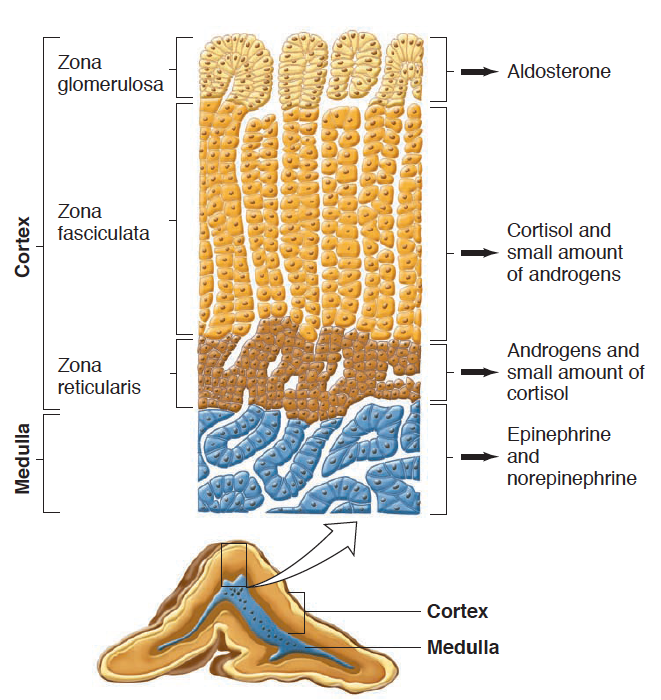
\includegraphics{figures/adrenal-anatomy}
  \caption{The anatomy of the adrenal gland.}
    \label{fig:adrenal-anatomy}
\end{marginfigure}

\section{Steroid Hormones Secreted from The Adrenal Gland}

Steroid hormones are synthesized from cholesterol via enzymes which are regulated by PKA signaling.  In response to the synthetic signal\sidenote{ACTH for cortisol; Angiotensin II for aldosterone}, the GPCR's are activated resulting in cAMP/PKA or IP3 signaling cascades.  Since steroid hormones are membrane soluble they can be released from the cell.  They move through the serum bound to proteins called globulins which keep them soluble in the blood stream.  Both aldosterone and cortisol signal via nuclear receptor signaling mechanisms in their target cells.

\subsection{Aldosterone}

Aldosterone, which is a mineralcorticoid is primarily responsible for sensing and modulating salt balance at the kidney.  It is produced in the adrenal cortex in a region called the zona glomerulosa.  The main site of action of aldosterone is the cortical collecting ducts and the distal convoluted tubule, where it functions to stimulate sodium re-absoroption.  

\newthought{The mineralcorticoid receptor} binds to aldosterone, which then promotes the transcription of three important genes involved in salt reuptake:

\begin{description}
 \item[Sodium/potassium pumps.]  These pumps exchange sodium for potassium, to move sodium out of the kidney and back into the blood.
 \item[ENac] This is a sodium transporter that helps get sodium from the tubule into the cells of the collecting duct.
 \item[SGK1] Is a protein kinase that activates several transporters by post-translational modification.
\end{description}

Together these genes when activated by aldosterone enhance the movement of sodium ions out of the kidney and back into the blood stream.  In the absence of aldosterone, the human body would secrete about 35g of sodium chloride per day.  When aldosterone levels are high (due to reduced sodium concentration), nearly all sodium is reabsorbed.  This complex system requires integration of information about blood volume, blood pressure and sympathetic activity.  This integrated endocrine circuite is known as the renin/angiotensin system

\begin{figure}
\centering
  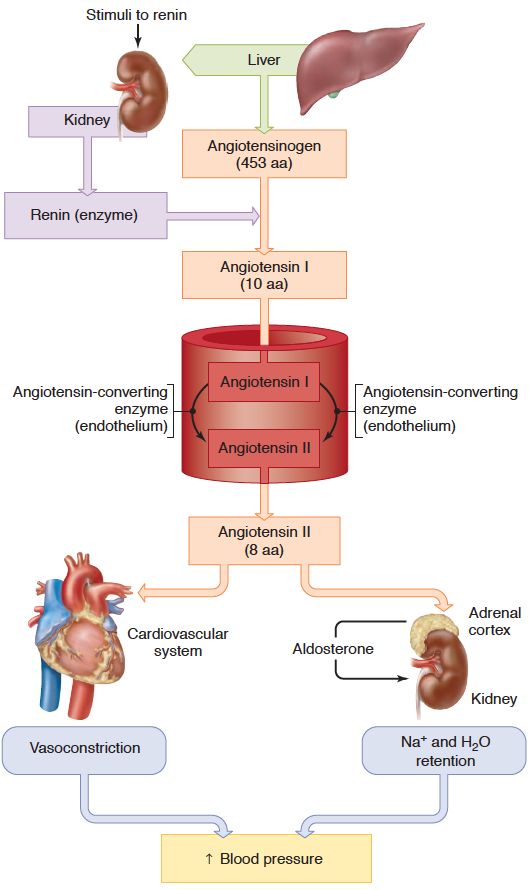
\includegraphics[width=0.5\textwidth]{figures/renin-angiotensin}
  \caption{The renin/angiotensin system.}
    \label{fig:renin-angiotensin}
\end{figure}

\newthought{The Reinin-Angiotensin system.} Angiotensin II\sidenote{the active form} is generated by the liver as a precursor molecule called angiotensinogen.  This molecule is processed in two stages to generate angiotensin II.  The first, and most important regulatory step is mediated by a secreted enzyme known as renin.  Renin is secreted from specialized pericytes near the kidney glomerulus known as juxtaglomerular cells\sidenote{JG cells, see Tigyi lectures for more information}.  When JG cells sense decreased stretch (decreased blood pressure), decreased glomerular flow or have elevated sympathetic nervous activity, Renin is released.  Renin converts angiotensinogen to angiotensin I, which in turn is converted to angiotensin II by angiotensin converting enzyme.  In this way, signaling to JG cells can cause increased angiotensin.  Angiotensin then causes increased vasoconstriction\sidenote{see lectures from O'Connell,  Mancarella and Adebiyi} and increased salt reuptake.  This pathway is illustrated in Figure \ref{fig:renin-angiotensin}.

\subsection{Cortisol}

PKA phosphorylates a protein called StAR which helps traffic cholesterol into the mitochondria where steroid hormone synthesis can begin.  

\newthought{Local concentrations of cortisol} are regulated by enzymatic inactivation by an enzyme known as 11$\beta$-hydroxysteroid dehydrogenase 2.

\section{Epinephrine and Norepinephrine}

\section{Pathophysiology Related to Adrenal Hormones}

\newthought{Cushings's disease is the result of elevated cortisol levels}, either due to a pituitary tumor which constitutively secretes ACTH, or an adrenal tumor which secretes too much Cortisol.

\newthought{Congenital Adrenal Hypertrophy\sidenote{also known as adrenogenital syndrome}} results from mutations in the biosynthesis genes involved in the production of steroid hormones.

\newthought{Addison's disease} is due to immune destruction of the adrenal gland, functionally also preventing steroid hormone production.

\listoffigures
\listoftables

\bibliography{library}
\bibliographystyle{plainnat}



\end{document}
